\section{Overview}
\label{sec:overview}

This section starts with the introduction of the NUMA architecture and potential performance issues. Then it briefly discusses the basic idea of \NP{} to identify such issues. 

\subsection{NUMA Architecture}
\label{sec:numa}

Traditional computers use the Uniform Memory Access (UMA) model. In this model,  all CPU cores share a single memory controller such that any core can access the memory with the same latency (uniformly). However, the UMA architecture cannot accommodate the increasing number of cores in recent years because these cores may compete for the same memory controller. The memory controller becomes the performance bottleneck in many-core machines since a task cannot proceed without getting its necessary data from the memory. 

\begin{figure}[htbp]
%\vspace{-0.1in}
\centering
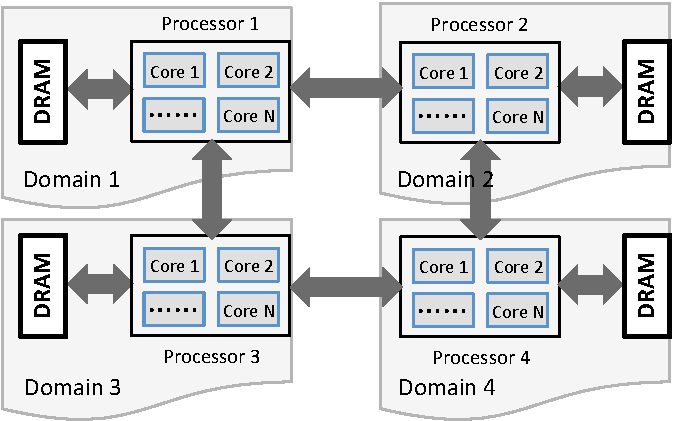
\includegraphics[width=0.9\columnwidth]{paper/figures/Numa.pdf}
\caption{An NUMA architecture with four nodes/domains\label{fig:numa}}
%\vspace{-0.1in}
\end{figure}
The Non-Uniform Memory Access (NUMA) architecture is proposed to solve this scalability issue, as further shown in Figure~\ref{fig:numa}. It has a decentralized nature. Instead of making all cores waiting for the same memory controller, the NUMA architecture  is typically equipped with multiple memory controllers, where each controller serves a group of CPU cores (called as a node or processor interchangeably). Incorporating multiple memory controllers largely reduce the contention for memory controllers and therefore improve the scalability correspondingly. However, the NUMA architecture also introduce multiple sources of performance degradations~\cite{Blagodurov:2011:CNC:2002181.2002182}, including \textit{Cache Contention}, \textit{Node Imbalance}, \textit{Interconnect Congestion}, and \textit{Remote Accesses}. 

\textbf{Cache Contention:} the NUMA architecture is prone to cache contention: multiple tasks may compete for the shared cache. Cache contention will cause more serious performance degradation if data has to be loaded from a remote node. 
 
\textbf{Node Imbalance:} When some memory controllers have much more memory accesses than others, it may cause the node imbalance issue. Therefore, some tasks may wait more time for memory accesses, thwarting the whole progress of a multithreaded application.  

\textbf{Interconnect Congestion:} Interconnect congestion occurs if some tasks are placed in remote nodes that may use the inter-node interconnection to access their memory. 

\textbf{Remote Accesses:} In NUMA architecture, local nodes can be accessed with less latency than remote accesses. Therefore, it is important to reduce remote accesses to improve the performance.\\


Based on an existing study~\cite{Blagodurov:2011:CNC:2002181.2002182}, node imbalance and interconnect congestion may have a larger performance impact than cache contention and remote accesses. These performance issues cannot be solved solely by hardware design. Software support is required to control the placement of tasks, physical pages, and objects to achieve the optimal performance for multithreaded applications.  
 
\subsection{Basic Idea}
\label{sec:idea}

% What is the major target: remote (false and true sharing, synchronization), load imbalance 

% Why we are using fine-grained, but not coarse-grained? Some issues are not able to identify when using the coarse-grained. For instance, duplication. 

% In order to detect the accesses, we will need to trace memory accesses. Then we are planning to utilize compiler-based instrumentation. Another option is to utilize binary-based instrumentation. 

As discussed in Section~\ref{sec:intro}, \NP{} has multiple design goals that separates it from existing work. First, \NP{} aims to design a topology-independent approach that could report performance issues in any NUMA hardware. Second, it aims to identify different sources of NUMA performance issues as discussed above, not just limited to remote accesses. Third, it aims to propose useful information to guide program fixes.  
%specific metrics to evaluate the seriousness of performance issues, instead of relying on programmers' judgement. 
%Therefore, there is no need to impose any additional runtime overhead in deployment environment. 


For the first goal, we have a key observation: \textit{a thread can be scheduled to any node, depending on the hardware topology or the scheduling}. Based on this observation, \NP{} proposes a \textbf{topology-independent} approach that overestimates the number of remote accesses: if a thread accesses a physical page that was initially accessed by a different thread, then this access can be a remote access.
Based on this, \NP{} tracks every access of each thread in order to identify the first thread working on each page. Due to this reason, \NP{} employs fine-grained instrumentation, instead of coarse-grained sampling. Since \NP{} focuses on thread's relationship, instead of node-relationship, which also reduces detection overhead by removing the checking on node-relationship. 

For the second goal, \NP{} detects NUMA issues caused by cache contention, node imbalance, interconnect congestion, and remote accesses, where existing work only considers remote accesses.  \textit{Cache contention} can be either caused by false or true sharing. False sharing occurs when different threads are accessing separate words in the same cache line~\cite{Hoard}. For both of them, when a thread alters any content of a cache line, the same cache line on other cores will be invalidated simultaneously,  forcing other threads accessing it reload the data. They may have a larger performance impact on the NUMA architecture, due to a higher latency of remote accesses. \NP{} will track all accesses in order to compute the number of cache invalidations with an overestimation. Note that  existing work does not consider false sharing and true sharing separately~\cite{XuNuma, valat:2018:numaprof}, but only consider remote accesses, which may miss some optimization opportunities, as shown in Table~\ref{tab:numa_issues}.  For \textit{node imbalance} and \textit{interconnect connection}, it is infeasible to measure them without knowing the actual memory and thread binding. Instead, \NP{} focuses on one type of issues that may easily introduce these issues, which is workload imbalance of different types of threads. \NP{} tracks the number of accesses to evaluate the workload imbalance and predict a good strategy for thread assignment.  For \textit{remote accesses}, existing work omits one type of remote accesses caused by thread migration, where thread migration will make all local accesses remotely. 
%Currently, the OS scheduler has no guarantee to put a thread into its original node, if a thread is blocked due to system calls or synchronization. Therefore,
\NP{} aims to identify applications with a higher chance of thread migrations, by checking the synchronization. A thread with the lock contention or invoking condition waits or barrier waits may pause the execution of the current thread, which may be scheduled to another node afterwards.  \NP{} then suggests thread binding to reduce remote accesses. For normal remote accesses, \NP{} tracks thread's relationship with pages to detect remote ones as discussed above. 

%However, we understand that putting closely-connected threads into the same physical node will reduce interconnect congestion. Then \NP{} aims to propose good thread clustering method that may reduce interconnect congestion. In particular, \NP{} employs the producer/consumer relationship between objects for the identification, as further described in Section~\ref{}.   

For the third goal, \NP{} will utilize the data-centric analysis as existing work~\cite{XuNuma}. That is, it could report the callsite of heap objects that may have NUMA performance issues. In contrast, another fine-grained profiler--NumaProf~\cite{valat:2018:numaprof}--could only report the lines of code that may access remotely, which require programmers to figure the specific object (i.e. the lines needs to be changed). In addition to that, \NP{} further provides useful information that helps bug fixes. It provides word-based access information on cache contentions, helping programmers to differentiate false or true sharing. It also reports whether an object can be duplicated or not by tracking the temporal read/write pattern, where only read-exclusively (after the first write) objects can be duplicated.  \NP{} also predicts a good thread assignment to achieve better performance for load imbalance issues. Overall, many of these features requires the fine-grained instrumentation in order to avoid false alarms, such as determining the duplication or false/true sharing. 


Based on the above discussion, \NP{} requires  fine-grained memory accesses to improve the effectiveness and provide better information for bug fixes. Based on that, \NP{} employs a compiler-based instrumentation in order to collect memory accesses, mainly due to the performance concern. An alternative approach is to employ binary-based dynamic instrumentation~\cite{DynamoRlO, Valgrind, Pin}, which may introduce more performance overhead but without an additional compilation step. \NP{} inserts an explicit function call for each read/write access on global variables and heap objects, while accesses on stack variables can be omitted since they typically do not introduce performance issues. To track thread migration, \NP{} also intercepts synchronizations. In summary, \NP{}'s basic idea is further explained in Figure~\ref{fig:overview}.  Basically, \NP{} includes two components, \NP{}-Static and \NP{}-Dynamic. \NP{}-Static is a static compile-time based tool that inserts function calls before memory accesses on heap and global variables, which compiles a program into an instrumented executable file. Then this execution file will be linked to \NP{}-Dynamic so that \NP{} could collect memory accesses,  synchronizations, and information of memory allocations. \NP{} then performs detection on NUMA-related performance issues, and reports to users in the end.  More specific implementations are further discussed in Section~\ref{sec:implementation}. 
\begin{figure}[htbp]
\centering
\includegraphics[width=0.98\columnwidth]{figures/overview.pdf}
\caption{Overview of \NP{}\label{fig:overview}}
%\vspace{-0.1in}
\end{figure}
